\chapter{John Horton Conway (1937-2020)}
\begin{wrapfigure}{r}{0.25\textwidth}
	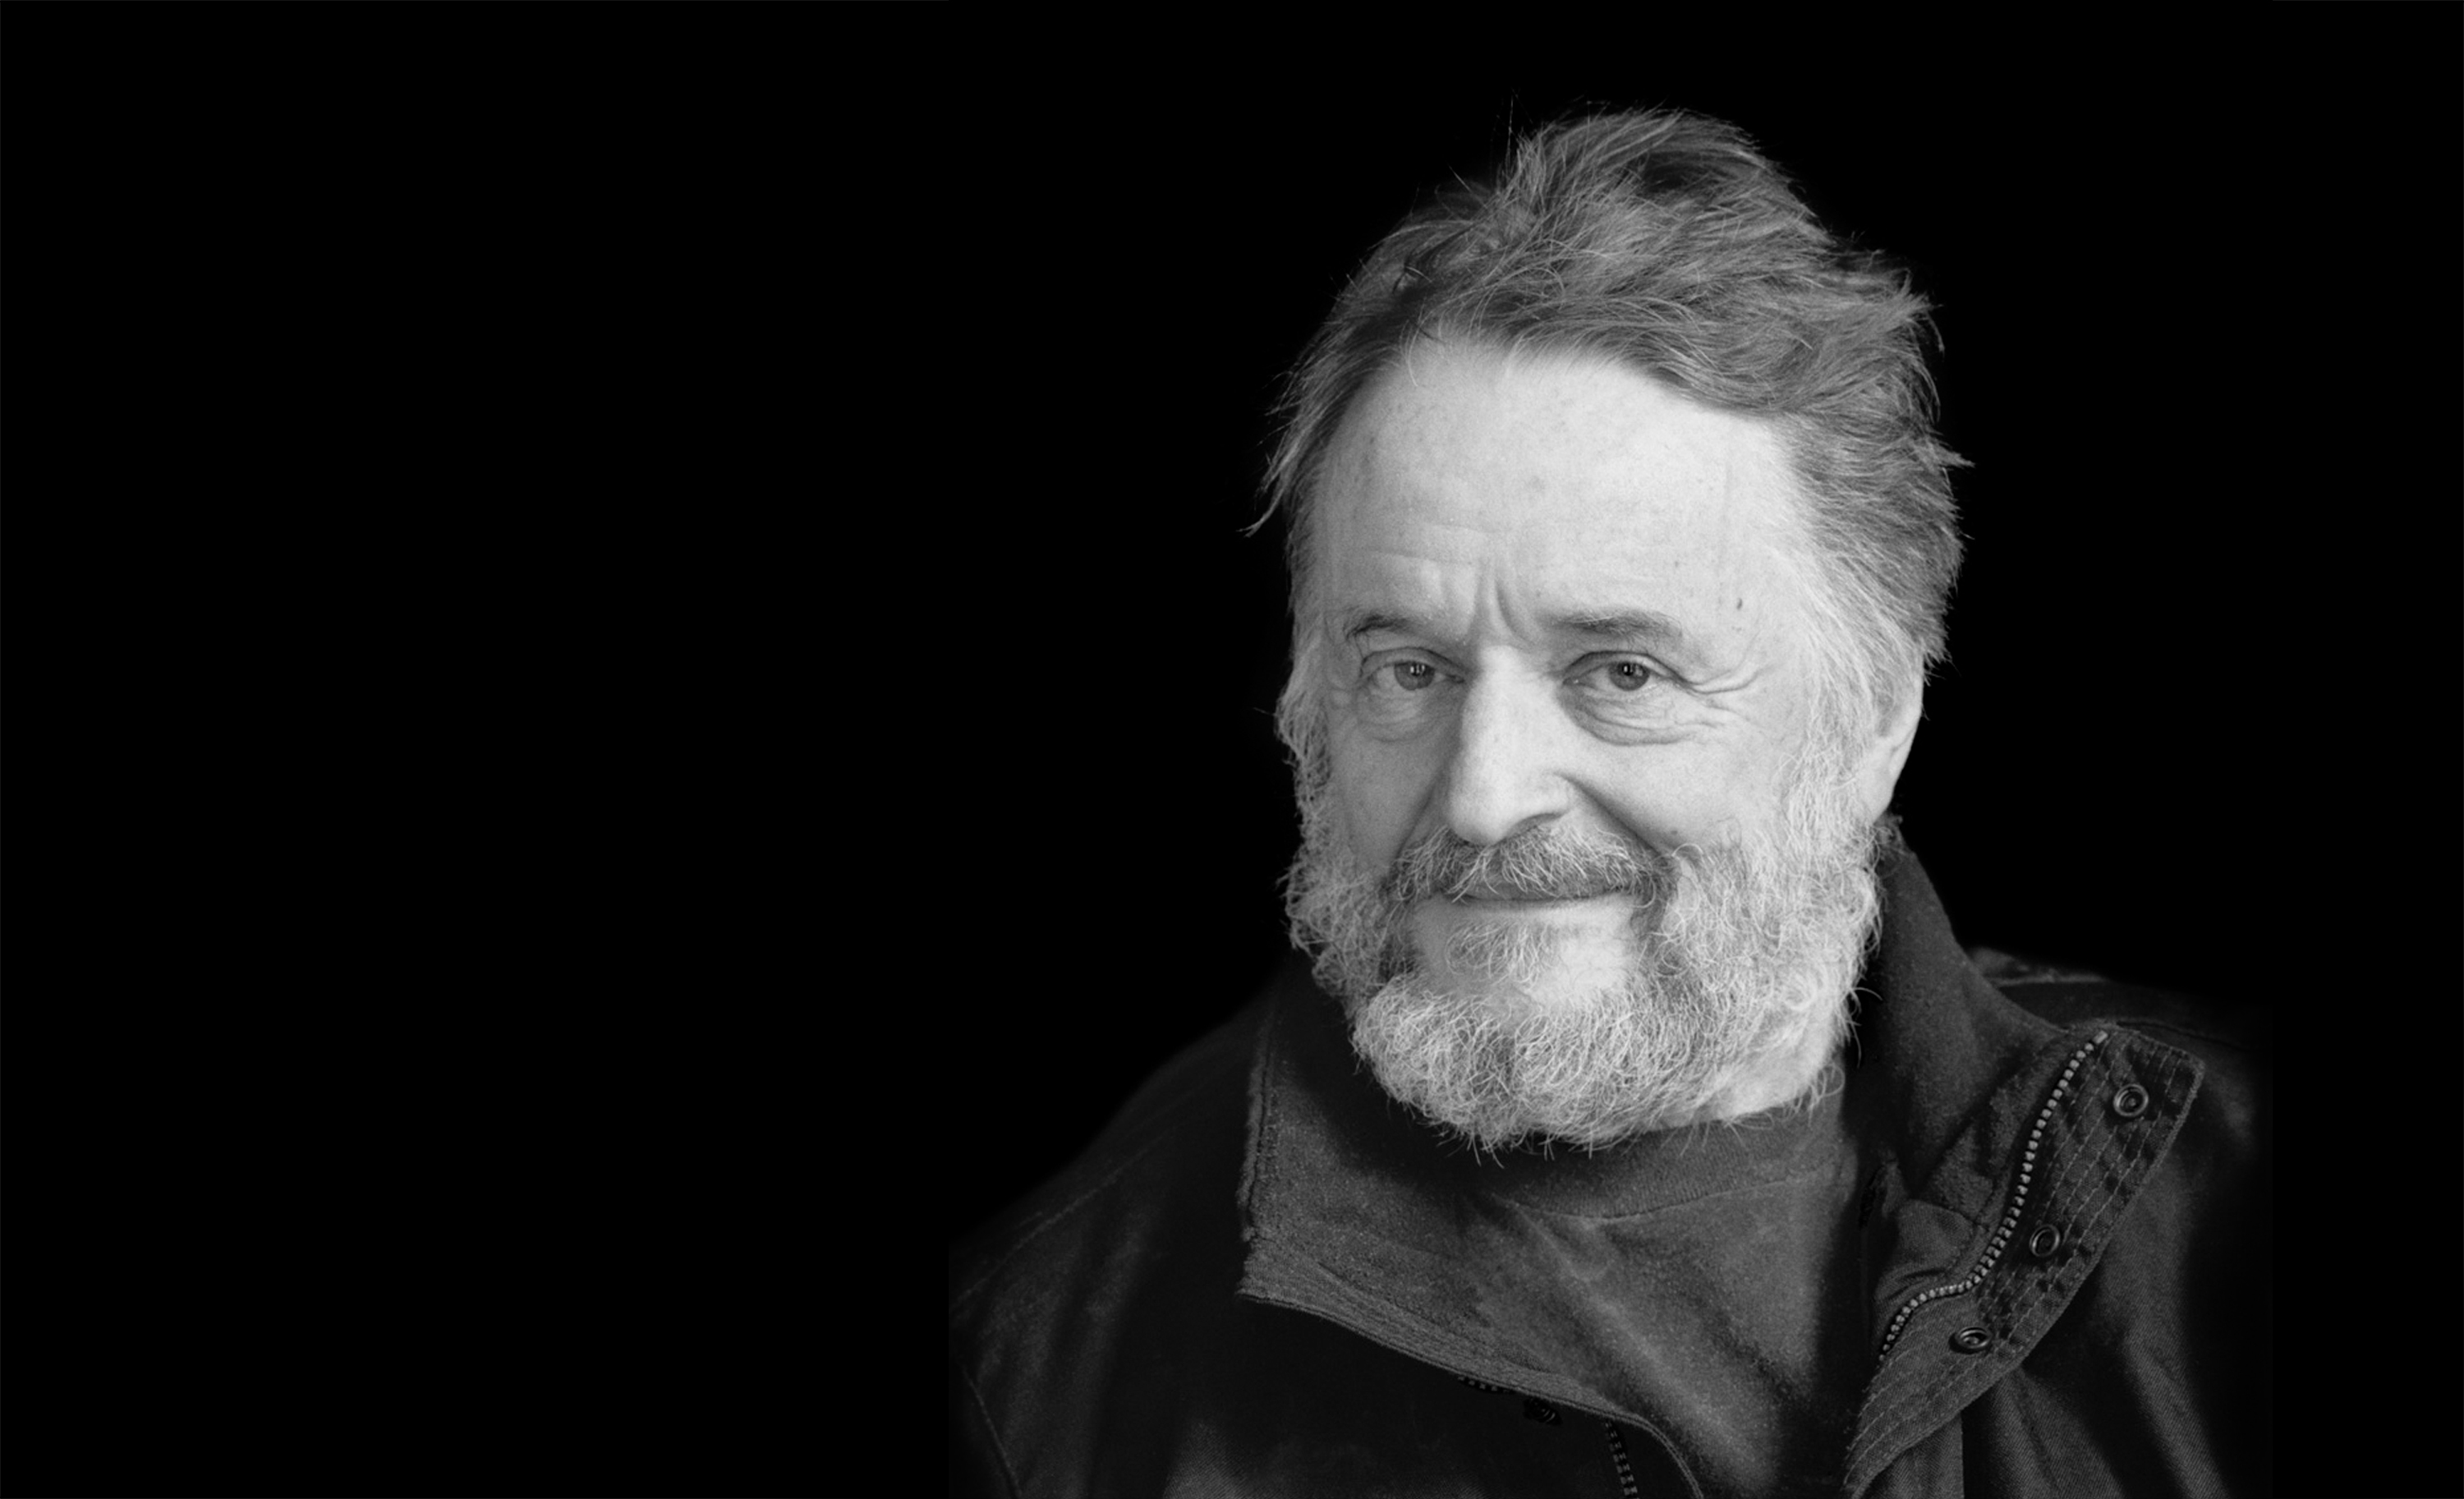
\includegraphics[width=0.3\textwidth]{capitulo1/images/conway.jpg}
\end{wrapfigure}

«Esta pequeña sección está dedicada a John Horton Conway, Por sus contribuciones a la matemática y particularmente por su conocido Juego de la vida que fue crucial para el entendimiento de lo que se conoce como emergent complexity o sistemas auto-organizables contribuyendo a lo que hoy se conoce como sistemas complejos.»
\\\\
John Conway hizo otras importantes contribuciones en teoría de grupos, teoría de números, álgebra, geometría, topología, teoría de nudos, combinatoria, teoría de juegos y física teórica entre otras. Fue autor de de más de 10 libros y cerca de 150 artículos de alto nivel. Siempre estuvo preocupado por difundir sus conocimientos no solo entre la comunidad matemática sino que realmente creía en la transdisciplinariedad y en ayudar a los más jóvenes, porque ellos son los encargados, en primera instancia, de hacer que se continúe en el progreso del conocimiento.

Como persona los que tuvieron la oportunidad de conocerlo incluyendo a quien sería autora de su biografía (Siobhan Roberts) coinciden en que era una persona muy amable a quien le encantaba contar historias e incapaz de contestar a una pregunta con un simple "sí"  \text{o} "no", era un genio, un gigante como muchos lo describieron, La universidad de Princeton a través de su sitio web dio la noticia de su lamentable fallecimiento, incluyendo un obituario de las personas que lo conocían personalmente,  De Diana Conway podemos leer esto: \textbf{“John fue el ser humano más fascinante que he conocido, él no solo estaba interesado en las matemáticas, estaba interesado en todo”.} \cite{princeton}
\\\\
La sucesión que se muestra a continuación es muy vista en páginas de acertijos o incluso he conocido personas que han tenido que programar para calcular el enésimo término, sin embargo pocos saben que esta sucesión tiene nombre propio: Sucesión de Conway:\\
$3, 13, 1113, 3113, 132113, 1113122113, 311311222113, …$



\chapter{Game of Life}

Game of Life o juego de la vida en español, es un autómata celular desarrollado por John Conway en 1970.
Consiste en una cuadrícula infinita de células cuadradas y su evolución es determinada solo por el estado inicial.\\\\
Las células pueden estar vivas o muertas, cada célula tiene 8 vecinas adyacentes.
\\
Las reglas son simples y describen la evolución de la cuadrícula:

\begin{itemize}
	\item \textbf{Nacimiento:} Una célula que está muerta en el tiempo $t$ estará viva en el tiempo $t+1$ si exactamente 3 de sus ocho vecinas estuvieron vivas en el tiempo $t$.
	\item \textbf{Muerte:} Una célula puede morir por:
		\begin{itemize}
			\item \textbf{Sobrepoblación:} Si una célula está viva en el tiempo $t$ y 4 o más de sus vecinas están también vivas en el tiempo $t$, la célula pasará a estar muerta en el tiempo $t+1$.
			\item \textbf{Soledad:} Si una célula viva en el tiempo $t$ solo tiene una vecina o ninguna vecina viva, estará muerta en el tiempo $t+1$.
		\end{itemize}
	\item \textbf{Supervivencia:} Una célula sobrevive del tiempo $t$ al tiempo $t+1$ si y solo sí 2 o 3 de sus vecinas están vivas en el tiempo $t$.
\end{itemize}
\newpage
\section{Patrones de Life}
\subsection{R-pentomino}
Inicia con 5 células, comienza a complicarse rápidamente, con este patrón se pueden descubrir algunos otros más simples.\\\\
El R-pentomino es el primer patrón que Conway encontró que desafió sus intentos por simularlo a mano. De hecho, el patrón eventualmente se vuelve 'estable' o fácil de predecir, pero esto no sucede sino hasta que han pasado 1103 unidades de tiempo. \cite{mitslides}
\begin{figure}[h]
	\centering
	
\includegraphics[width=0.1\textwidth]{capitulo1/images/rp.png}
	\caption{R-pentomino}
	\label{fig:pentomino}
\end{figure}
\subsection{Objetos Still Life}
Algunos de los objetos más comunes en el juego de la vida permanecen igual en cada paso. Ninguna célula viva muere y no nacen nuevas células. Conway llamó a este tipo de  objetos Still Life.
El más común de ellos es simplemente un cuadrado de 2x2 células vivas. \cite{mathpaul}

\begin{figure}[h]
	\centering
	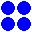
\includegraphics[width=0.07\textwidth]{capitulo1/images/block.png}
	\caption{Block}
	\label{fig:block}
\end{figure}

Algunos otros tipos de Still Life que se pueden encontrar se muestran en la siguiente Figura.

\begin{figure}
	\centering
	\subfigure[]{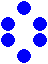
\includegraphics[width=0.1\textwidth]{capitulo1/images/beehive.png}} 
	\subfigure[]{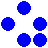
\includegraphics[width=0.1\textwidth]{capitulo1/images/boat.png}} \\
	\subfigure[]{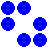
\includegraphics[width=0.1\textwidth]{capitulo1/images/ship.png}} 
	\subfigure[]{
\includegraphics[width=0.1\textwidth]{capitulo1/images/loaf.png}} 
	\caption{(a) Beehive (b) Boat (c) Ship (d) Loaf}
	\label{fig:still_life}
\end{figure}
\newpage
\subsection{Oscillators}
Los osciladores son objetos que cambian de un paso al otro, pero eventualmente se repiten. El tipo más simple es el oscillator de periodo 2, o aquellos que se repiten después de dos pasos. El más común es el blinker, que consiste de 3 células.

\begin{figure}[h]
	\centering
	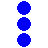
\includegraphics[width=0.07\textwidth]{capitulo1/images/blinker.png}
	\caption{Blinker}
	\label{fig:blinker}
\end{figure}
Otro oscillator es el Toad, que también aparece en el R-pentomino después de 737 pasos, es destruido por una explosión después de solo 14 pasos.
\begin{figure}[h]
	\centering
	
\includegraphics[width=0.07\textwidth]{capitulo1/images/toad.png}
	\caption{Toad}
	\label{fig:toad}
\end{figure}
\newpage
\subsection{Gliders	}
Uno de los descubrimientos más emocionantes que se encontraron primero en el juego de la vida son los objetos que se mueven. Estos patrones en movimiento se llaman gliders.\\
Los gliders se repiten cada 4 generaciones, pero se desplaza diagonalmente una célula.

\begin{figure}[h]
	\centering
	
\includegraphics[width=0.07\textwidth]{capitulo1/images/glider.png}
	\caption{Glider}
	\label{fig:glider}
\end{figure}

\subsection{The Queen Bee Shuttle}
Un patrón muy importante que aparece después de correr el R-pentomino durante 774 unidades de tiempo es \textbf{The Queen Bee Shuttle}.

\begin{figure}[h]
	\centering
	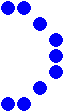
\includegraphics[width=0.07\textwidth]{capitulo1/images/queen.png}
	\caption{The Queen Bee Shuttle}
	\label{fig:bee}
\end{figure}
Aunque en el entorno del R-pentomino no dura mucho tiempo, por sí sola primero se mueve a la derecha, pero después de unos pocos pasos, se produce un Still Life llamado Beehive a su izquierda y se da la vuelta de nuevo. Conway la nombró.\textbf{The Queen Bee Shuttle}. por esta razón. Aunque después choca en la siguiente unidad de tiempo con la primer Behive que creó.\\\\
Existen otros patrones no presentes en el R-Pentomino como The orthogonal spaceships  en \cite{mathpaul}.